\section{Szimulációs vizsgálat (Szorgalmi feladat)}
Az egyenáramú motor folytonos modelljét terhelőnyomaték beiktatásával is szimuláltam. Mivel az eredeti feladat Matlab/Simulink környezetet írt elő, a megfelelő folytonos egyenleteket (StateSpace) Python \texttt{scipy.signal} könyvtárral oldottam meg pontos formában. A névleges feszültség ugrása és egy egyidejű $0.01$ Nm lassító terhelés hatására a kialakuló válasz a következő:
\begin{figure}[H]
    \centering
    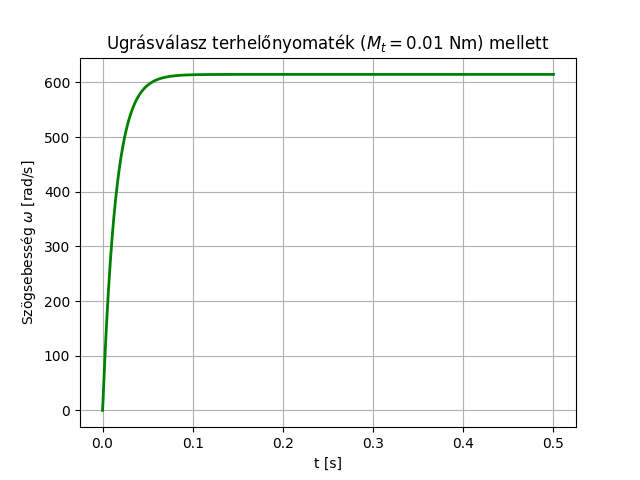
\includegraphics[width=0.8\textwidth]{res/imgs/fig_Szorgalmi.png}
    \caption{Ugrásválasz bekapcsolt $0.01$ Nm terhelőnyomaték mellett}
\end{figure}
Az állandósult érték értelemszerűen alacsonyabbra adódik, mint terheletlen esetben a lassító nyomatéki igénybevétel miatt.
